%
%\section{Building and verifying assembly-level refinements}
%\label{sec:studycase}


This section shows a case study that carries an out experimental evaluation of
a pilot project with B refinements until the assembly level. The object of
the pilot project was developed to analyse a petroleum production test system.  

%A seção 1 apresenta uma introdução sobre o sistema de teste de produção em tanque e a seção seguinte
%descreve a modelagem B e B \textit{assembly}. A seção 3 mostra a simulação do \textit{software}
%desenvolvido, o que foi realizado para testar o seu funcionamento. Finalmente, a última seção 
%apresenta as considerações finais sobre a modelagem desse estudo de caso.


\subsection{Petroleum production test system}

%\subsection{Teste de produção em tanque}

% Intro % O que é isso ?
%O teste de produção é ``o processo usado para o acompanhamento do desenvolvimento da produção de um
%campo de petróleo, o qual é executado em cada poço deste campo numa frequência previamente definida''
%\cite{LAUT_SERGIO}. Nesse processo são analisadas as características do óleo, gás e água extraídos, tais como:
%volume, concentração de água, temperatura, entre outras.	

The production test is ``the process used to  monitor the production of an oil
field, this process is executed in each oil field in a predefined frequency''
according to \cite{LAUT_SERGIO}. In this process, some characteristics
are analysed (concentration of water, volume and temperature) from oil, gas and
water.

%% Porque modelar isso ? O que pode melhorar ?
%Esse tipo de teste possui um papel importante no processo de extração. Ele é fundamental
%para avaliar a capacidade de extração dos poços e para designar o pagamento dos impostos governamentais, o pagamento de \textit{royalties} aos
%municípios, as participações especiais e as participações aos proprietários de terra. No entanto,
%atualmente, segundo registros dos testes no sistema de informação, 10\% deles são falhos~\cite{LAUT_SERGIO}. Logo, é importante que
%esses testes obtenham a melhor precisão possível, a fim de garantir uma melhor qualidade, credibilidade e
%transparência.


This production test system has an important purpose in the process of oil
extraction. It is required to analyse the production capacity of wells and
calculate the government taxes, special participations and participations for
landowners. However, based on the registers of the information system test,
10\% of production tests are failed tests~\cite{LAUT_SERGIO}. So, we have developed an embedded
software verified until the assembly level to help the production test. Actually,
the developed software is simplified, because its main objective is to evaluate
and to improve the verification up to the assembly level.



% Simplificação/abstração de detalhes não relevantes
%O sistema de teste de produção é utilizado para controlar e avaliar a produção de petróleo. Ele possui um
%sistema supervisório que calcula a produção de petróleo e controla as válvulas de acordo com os estados do
%sistema, do sensor de interface e do radar. O radar informa o nível total do fluido no tanque e o
%sensor de interface informa a concentração de água na emulsão em um ponto local independente da
%densidade, viscosidade e temperatura de operação, o que ajuda a identificação do nível da interface. Esse sistema é complexo
%e pode ser considerado sob vários pontos de vista, no entanto, ele é simplificado nessa proposta até o nível de abstração
%adequado para facilitar o entendimento. 

%Uma série de técnicas e cuidados físicos deve ser aplicada para realização correta dos testes de produção. Dessa forma, o sistema de teste
%envolve uma considerável complexidade. Além disso, os trabalhos de~\cite{LAUT_SERGIO,LAUT_LIMA} definem vários
%detalhes físicos e parámetros para melhorar a qualidade dos testes, os quais foram obtidos e aprimorados após
%experimentos em campo. Esses detalhes podem ser consultados nos trabalhos citados, e nesse trabalho é
%apresentada apenas uma visão geral do problema e a especificação de uma parte do sistema.

The production test system is used to control and to evaluate the oil production.
It has a system supervisor that calculates the oil production and controls the
valves based on the state of system and information from sensor interface and
radar. The radar informs the total level of fluid in the tank and the interface sensor
informs the concentration of water in oil that helps to identify the level of
interface oil and water.
% Several physical precautions and techniques can be applied to execute correctly
% the production system test.




% % Como funciona o estudo de caso?
% O teste de produção, resumidamente, possui três fases de acordo
% com~\cite{LAUT_SERGIO}. Primeiramente, inicia a fase de condicionamento, o
% sistema de controle do tanque é atualizado com dados coletados do último teste,
% o sistema mantêm o poço alinhado\footnote{Um poço está alinhado quando as
% válvulas da tubulação direcionam o fluxo do poço para o tanque.} e ao final dessa fase a válvula de drenagem é fechada.


The production test has basically three stages according to~\cite{LAUT_SERGIO}.
First, the conditioning stages begin, the control system of the tank is updated
with data collected from the last test, the system keeps the well
aligned\footnote{A well is aligned when the valves direct the flow pipe from the
well to the tank.} and the drain valve is closed in the end of this stage.

% Em seguida, inicia a fase de enchimento e decantação, logo após o enchimento e
% a espera, que pode variar de 8 a 20 horas de decantação, começa a fase de
% drenagem. Nessa última fase, o sistema deve
% controlar a válvula de drenagem para não permitir fluir o óleo extraído e calcular a sua quantidade.
% E esse cálculo é o objeto de interesse do presente estudo de caso.

Then the process of filling and decanting begins. After filling and waiting,
which can wait between 8 and 20 hours of decanting, the draining stage begins.
The draining stage is on that last one stage, the system must control the drain valve
not to allow the extracted oil to flow and to estimate final quantity oil. Only
the calculus used to estimate oil quantity in this last stage is important to the
case study verified up to assembly level.

%As três fases citadas são exibidas na mesma ordem na Figura~\ref{fig:CaseStudy}. Nessa figura é
%possível observar os dispositivos utilizados no teste de produção e os estados do tanque
%em cada fase.
The three stages are shown, in the same sequence, in Figure~\ref{fig:CaseStudy}.
In this Figure, it is also possible to see the used devices in the production
test.

\begin{figure}[h] \centering 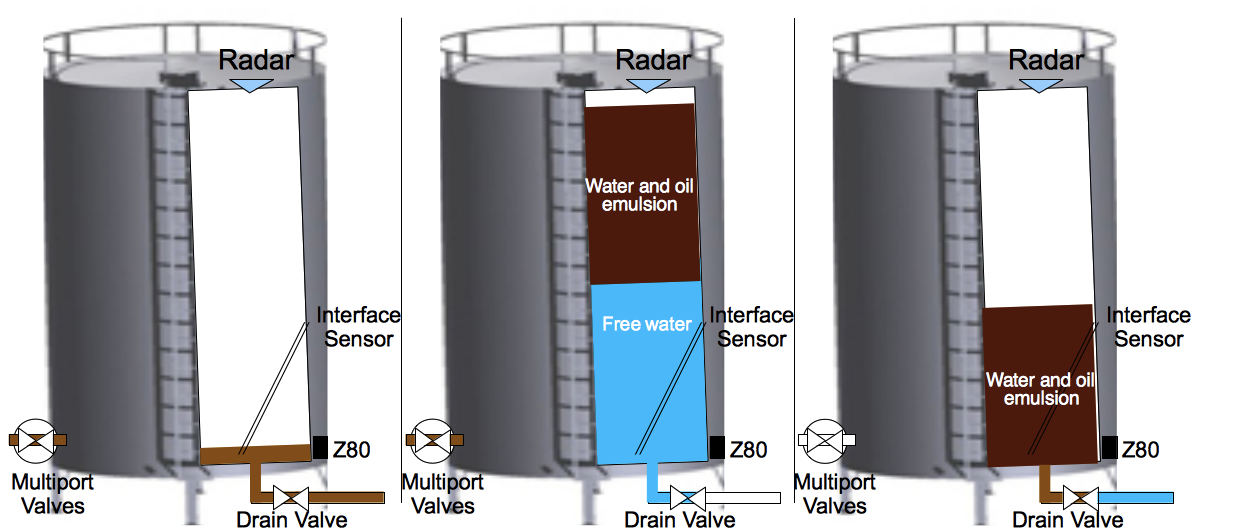
\includegraphics[width=1.\textwidth]{images/FasesEstudoDeCaso.png}
\caption{Stages of the production test.}
\label{fig:CaseStudy}
\end{figure}

% Na fase de drenagem, o nível de óleo desce relativamente rápido até aproximar-se do sensor de interface.
% Nesse instante a válvula de drenagem começa a fechar lentamente e, consequentemente, diminui a
% velocidade de  saída do fluido. Todo esse cuidado é importante para evitar a formação de vórtice\footnote{Vórtice
% é disposição concêntrica e raiada do fluido, ou seja, redemoinho ou pequenas
% ondas.}, o que afeta diretamente as propriedades do óleo extraído.


% [Dúvidas]
% - O sistema de automação usa clp (microcontrolador), ok? Sim Onde? No controle da válvulas, no recebimento das
% informações e cálculo de nível. Mais detalhes podem ser obtidos na dissertacao de LIMA
% - O  computador supervisório ? Apenas monitora e envia comandos! O microcontrolador é quem trabalha mesmo! Mais
% metalhes na {LAUT_LIMA}
% - 

%\begin{figure}[h]
%\centering 
%\includegraphics[width=.8\textwidth]{images/fluxograma_teste_drenagem.png}
%\includegraphics[width=0.95\textwidth]{images/diagrama_de_atividades.png}
%\caption{Diagrama de atividades do sistema de controle da válvula de drenagem do teste de produção
%\cite{LAUT_SERGIO}.}

%\label{fig:FluxogramaEstudoDeCaso}
%\end{figure}

%A Figura~\ref{fig:FluxogramaEstudoDeCaso} mostra o diagrama de atividades sobre o sistema de controle da
%válvula de drenagem.
% Contudo, para melhor entender o diagrama é necessário conhecer alguns conceitos: BSW
%é a abreviação de \textit{Basic Sediments and Water} e mede a proporção de água e sedimentos no fluído
%extraído; BSWe mede a proporção do volume de água contido na emulsão água e óleo entre o volume total
%dessa emulsão; CW (\textit{cut water}) representa a capacidade do óleo emulsionado reter mais ou menos
%água. De acordo com \cite{LAUT_SERGIO}, o CW é definido no programa como 20\% ou 40\%, conforme a
%densidade do fluido; e esses valores foram pré-definidos após experimentos em campo. O sistema de controle
%da válvula de drenagem começa inicializando as variáveis do sistema, esses valores são ajustados de acordo
%com o teste realizado anteriormente e experimentos. Em seguida, o sistema passa a monitorar o estado do
%sensor e do radar. O sistema vai ajustando lentamente o nível de abertura da válvula de drenagem até o
%sensor de interface identificar óleo. Finalmente, o processo de teste termina.

% Paragrafo de acima adaptado em baixo

%Para melhor entender a fase de drenagem é importante conhecer o conceito de
%BSW, a abreviação de
%\textit{Basic Sediments and Water}, que representa a proporção de água e
%sedimentos no fluído extraído.
%; BSWe
%mede a proporção do volume de água contido na emulsão água e óleo entre o volume total dessa emulsão;
% CW (\textit{cut water}) representa a capacidade do óleo emulsionado reter mais ou menos água. De acordo
% com \cite{LAUT_SERGIO}, o CW é definido no programa como 20\% ou 40\%, conforme a densidade do fluido; e
% esses valores foram pré-definidos após experimentos em campo.
%De acordo com o valor do BSW histórico do poço e outras propriedades do
%fluído, o sistema estima o nível da interface água e óleo.
% O sistema de controle da válvula de drenagem começa inicializando as variáveis do sistema, esses valores
% são ajustados de acordo com o teste realizado anteriormente e experimentos.
%Em seguida, o sistema passa a controlar a válvula de drenagem e a monitorar o
%estado do sensor e do radar. O sistema vai ajustando lentamente o nível de
%abertura da válvula de drenagem até o sensor de interface identificar a emulsão
%água e óleo. Finalmente, o processo de teste termina.

% % Motivação para o que pretendemos modelar
% Como uma medição exata reduz sensivelmente a margem de erro,
% a técnica desenvolvida por \cite{LAUT_SERGIO} pretende identificar com boa
% exatidão o atual nível da lámina de óleo através das informações seguintes:
% valor do sensor de interface,  ní­vel do tanque obtido pelo radar e outros
% parâmetros obtidos através de experimentos. Porém, uma garantia matemática sobre
% o correto funcionamento do sistema é fundamental. Assim, um cuidado especial deve ser
% realizado nesse sistema.

% % De que forma ?  O sistema verificado pode atuar ? Como um sistema redundante, visto o grau de confiança
% Para essa finalidade, um \textit{software} foi especificado, verificado, implementado e simulado. A princípio, o \textit{software}
% desenvolvido pode atuar como um sistema redundante na plataforma Z80 para interagir com os dispositivos e o sistema supervisório.
% Esse \textit{software} apenas realiza um cálculo relativo a produção de óleo, com a finalidade de avaliar se o sistema está funcionando corretamente.


B models were created to represent partially the production test system. This
report shows, in \ref{sec:Bmodel_case_study},  the main part of specification
system is organized in three different B models: \textit{TestCalc},
\textit{TestCalc\_i} and \textit{TestCalc\_basm}.

%  This specification is small and simplified, because its main objective
% is to demonstrate the technique of verification up to assembly level.

% O que pretende-se modelar ? O que foi feito ?
%Assim, o software foi implementado em \textit{assembly} e simulado um
%\textit{software} para calcular um fator de proporção de óleo bruto e água livre.

% Aparentemente, o projeto de desenvolvimento desse \textit{software} é uma atividade relativamente simples,
% porém como a técnica de verificação utilizada até o nível de \textit{assembly} é completamente inovadora,
% então surgiram algumas dificuldades iniciais que levaram tempo para ser solucionadas. A seção seguinte
% apresenta mais detalhes sobre a modelagem desse \textit{software}. 
% Essas funcionalidades foram modeladas em B
% e apresentadas nas duas seções seguintes.




%[explicar as conexão/comunicação entre os dispositivos]
 % Para realizar a comunicação entre os dispositivos serão utilizados conversores analógico/digital. 
 % As informações estão representanda em 8 bits.
 % Explicar o Wait bit de espera :D

% \subsection{Modelagem B do controle da válvula de drenagem}
% \label{sec:Modelagem B do controle da válvula de drenagem}
% 
% %[Explicar o objetivo do modelo]- princ
% [Rascunho]
% O obejtivo principal da modelagem apresentada nesta seção é especificar a parte essencial do controle da
% válvula de drenagem. Como visto anteriormente na fase de drenagem, essa válula  varia o
% estado de abertura de acordo com dois critérios: o nível da lámina de óleo ou sensor de interface, o qual 
% identifica óleo ou água no fundo do tanque. Considerando que se o sensor de interface
% indica a presença de óleo, então o sistema deve fechar a válvula do dreno. Caso contrário, ou seja,
% indica a presença de água livre, então o sistema deve ajustar a abertura da válvula proporcionalmente ao
% nível de água livre.
% 
% 
% % O software que faz controle da válvula de drenagem pode ser separado em três partes:
% % Cálculo do nível inicial ( multiplicação e condicional \ldots )
% % Atualização do nível inicial ( Uma subtração e atualização da variável )
% % Controle da abertura da válvula ( Atualização do controle da válvula )
% % A modelagem dessa seção preocupa-se com o controle da válvula de abertura.
% 
% 
% Como visto na Figura \ref{fig:FluxogramaEstudoDeCaso} o valor da válvula é atualizado aproximadamente em
% intervalos de 15 cm. Contudo, segundo \cite{LAUT_SERGIO}  é sugerido o uso de uma função do tipo rampa
% $valve=k*t$, a fim de evitar fechamentos bruscos. Onde, $valve$ é o percentual de abertura, $k$ é uma
% constante e $t$ é o tempo. Baseado na função utilizada atualmente, sugiro a seguinte função: $valve = k*H
% + c1$. Onde, $H$ é o nível de água livre, $k$ é igual à  $0,5$ e $c1$ é uma constante para abertura
% adicional, o qual pode ser ajustado para evitar um tempo excessivo no processo de drenagem. 
% 
% A Figura~\ref{fig:GraficoFuncoes} ilustra as funções de controle da válvula de drenagem, o eixo vertical
% representa o percentual de abertura da válvula de drenagem e o eixo horizontal representa $H$ (o nível de
% água livre), o que é inversamente proporcional ao tempo de drenagem.
% 
% A função representada em linha azul é a utilizada atualmente, a mesma descrita na Figura 
% \ref{fig:FluxogramaEstudoDeCaso}. A representada em linha vermelha é a proposta por esse trabalho, essa
% possui uma maior abertura inicial (100\%) e fechamento mais suave, o que reduz o tempo de
% drenagem e evita a formação de vórtice.
% 
% 
% \begin{figure}[h]
% \centering 
% %\includegraphics[width=.8\textwidth]{images/fluxograma_teste_drenagem.png}
% \includegraphics[width=0.99\textwidth]{images/Grafico_funcoes_da_valvula.png}
% \caption{Gráfico das funções que controla a válvula de drenagem..}
% 
% \label{fig:GraficoFuncoes}
% \end{figure}
% 
% Manipulando a função ($valve = 0.5*H + c1$) e substituindo $H$ pelo parámetro $level$ temos a seguinte
% função $valve = level/2 + c1$. O sistema também deve levar em consideração a informação obtida pelo
% sensor de interface, o que informa a presença de água livre no fundo do tanque. Dessa forma, a operação
% B seguinte modela essa funcionalidade. A operação ``ControlValve'' recebe como parámetro o nível de água
% livre ($level$) e o parámetro ($water$) para calcular a abertura da válvula de drenagem adequada.
% 
% \begin{tabular}[c]{l}
% \hspace*{0.20in}\bf ControlValve\rm (\it level\rm , \it water\rm )\rm =\\
% \hspace*{0.20in}\bf PRE\\
% \hspace*{0.40in}\it level\hspace*{0.10in} $\in$  \rm 0 $\upto$ \rm 2\rm 0\rm 0  $\land$  \it water 
% $\in$  \rm 0 $\upto$ \rm 1\\
% \hspace*{0.20in}\bf THEN\\
% \hspace*{0.40in}\bf IF \it water \rm = \rm 1 \bf THEN \it valve \rm := \it level $\div$ \rm 2 \rm + \it
% c1\\
% \hspace*{0.40in}\bf ELSE \it valve\rm :=\rm 0 \bf END\\
% \hspace*{0.20in}\bf END
% \end{tabular}
% 
% O primeiro refinamento dessa operação para o nível de assembly é representado a seguir no texto.
% Um fato interessante é que ele aproveita-se da propriedade da representação em \textit{bits}. Essa
% propriedade diz que a rotação à  direita de um vetor de bits é semánticamente equivalente à  divisão por
% $2^{n}$, onde $n$ é o número de rotações. Na operação de rotação $\textit{rotateright}$ $n$ é igual à  1,
% porém essa é uma rotação circular, ou seja, o bit menos significativo é copiado para o bit mais
% significativo. Para tornar a equivalente à  divisão por dois é o bit mais significativo é zerado através
% da função $\textit{bitclear}$.
% 
% \begin{tabular}[c]{l}
% \hspace*{0.15in}\bf ControlValve \rm ( \it level \rm , \it water \rm ) \rm =\\
% \hspace*{0.15in}\bf PRE\\
% \hspace*{0.35in}\it level  $\in$  \rm 0  $\upto$  \rm 2\rm 5\rm 5  $\land$  \it water  $\in$  \rm 0 
% $\upto$  \rm 1\\
% \hspace*{0.15in}\bf THEN\\
% \hspace*{0.35in}\bf IF \it water \rm = \rm 1\\
% \hspace*{0.35in}\bf THEN\\
% \hspace*{0.55in}\bf IF \it level  $\in$  \rm 2\rm 0\rm 1 $\upto$ \rm 2\rm 5\rm 5 \bf THEN \it valve\rm
% :=\rm 1\rm 0\rm 0\\
% \hspace*{0.55in}\bf ELSE \it valve \rm := \it byte\_uchar\rm (\it bitclear\rm (\it rotateright\rm (\it
% uchar\_byte\rm (\it level\rm )\rm )\rm ,\rm 7\rm )\rm )\rm +\it c1 \\
% \hspace*{0.55in}\bf END\\
%  \hspace*{0.35in}\bf ELSE\\
% \hspace*{0.55in}\it valve \rm := \rm 0\\
% \hspace*{0.35in}\bf END\\
% \hspace*{0.15in}\bf END\\
% \end{tabular}
% 
% 
% A seguir é ilustrado o modelo em nível de assembly. 
% \begin{tabular}[c]{l}
% \ldots
% \end{tabular}
% 
% 
% Esse cógigo assembly foi simulado em \cite{Simulator_z80}. A Figura\ref{fig:control_valvula} ilustra o
% final da execução os valores de entrada \ldots e saída \ldots
% 
% \begin{figure}[h]
% \centering 
% \includegraphics[width=0.45\textwidth]{images/Simulator_main.png}
% \includegraphics[width=0.45\textwidth]{images/Simulator_Execution.png}
% \includegraphics[width=0.45\textwidth]{images/Simulator_IO_ports.png}
% \includegraphics[width=0.45\textwidth]{images/Simulator_Peripheral_Devices.png}
% \caption{Simulação do controle da válvula de drenagem.}
% \label{fig:control_valvula}
% \end{figure}
% 
% 
% 
% [abstrações]- princ 
% 
% [explicar a modelagem]
% Quais as entradas e saídas do programa ?
% [Colocar as images de simulação do Z80]
% [explicar as estátisticas] [Explicar as dificuldades] 
% [explicar as regras utilizadas]
% % DICAS PARA DISSERTAÇÃO
% % 
% % -> Explicar uma das maiores dificuldades atuais! Que é a pouca simplificação realizada, o histórico que é mantido!
% % A simplificação das expressões poderia ser mais específica. As regras de simplificação utilizadas no AtelierB muitas vezes perdem "informações importantes".
% % [Colocar um exemplo pequeno antes da simplificação e após a simplificação.]
% % 
% % Existem duas solu
% % - Simplifificar utilizando novas regras
% % - Utilizar o ambiente do ABTools e aproveitar o gerador de obrigações de prova e simplificar as expressões.
% % 
% % 
% % Vantagens em calcular somente o nível:
% % - Pode-se se adequar a qualquer tamanho de tanque.
% % Assim, o nível e o determinado tanque que deve informar a quantidade de óleo produzido.
% % 
% % Posso pegar as obrigações de prova e tentar explicar o que é provado!?!
% % * Na documentação colocar o número de provas óbvias e não obvias
% % 
% % -> Na conclusão colocar o número total de obrigações de provas não obvias realizadas!!!

\subsection{B modelling} 
%e o \textit{software} do cálculo dos fatores de óleo bruto e água livre produzidos}
\label{sec:Bmodel_case_study}

% Overview 
% [Explicar o objetivo do modelo]- princ
% [explicar a modelagem]
% - inicial, implementação, explicar o que refinamento garante,  e assembly código, explicar o
% invariante, as entradas e saidas.
% [explicar as estátisticas]
% [Processo de prova](Pouca coisa,algumas linhas) citar o comando que resolveu 465 automaticamente entre
% 568, é explicado em anexo.
% [Simulação]
% Explicar as images, a entrada e saída \ldots
% [Conclusões]
%
 

% % Overview A presente seção apresenta a modelagem B e o \textit{software} do
% cálculo do fator de proporção de óleo bruto (emulsão água e óleo) e  água livre
% produzidos.

This section shows the B modelling and the embedded software that calculates the
proportion of water and oil emulsion produced.

% % [Ressalva -> onde tiver nível substituir por proporção]
% Os fatores de proporção de óleo bruto e água livre são determinados através de informações obtidas na
% fase de drenagem. As informações utilizadas são os níveis do tanque: inicial (tanque cheio) e final (tanque com
% apenas óleo bruto) da fase de drenagem.Portanto, a subtração desse dois valores determina um fator de
% proporção de água livre produzida e o nível final do tanque determina um fator de proporção de óleo bruto
% produzido.Para determinar exatamente a quantidade de óleo e água livre, é necessário que o resultado
% seja multiplicado por um fator de correção, o qual deve representar as distorções e o formato do tanque,
% já que o tanque não tem um formato perfeitamente cilíndrico. Dessa forma, esse \textit{software}
% embarcado torna-se genérico para qualquer formato de tanque.

The proportion of factors of water and oil emulsion are estimated by collected
information in the draining stage. The information used are the levels of the
tank: initial level (full tank) and final level (tank with only water and oil
emulsion) from draining stage. So, the subtraction of two values determines a
proportional factor of free water proportion and the final level of tank
determines a proportional factor of produced water and oil emulsion (crude oil).
To determine exactly the quantity of oil emulsion and water free, it is needed to
multiply the levels by the correction factor, which represents the format of the
tank and its deformations, because the tank has not a perfectly cylindrical
shape. Thus, the final embedded software becomes generic for any tank shapes.


% Modelagem funcional
% A modelagem é iniciada com o modelo funcional \textit{TestCalc}. Esse modelo contém duas variáveis
% \textit{oil\_factor} e \textit{free\_water\_factor} que representam respectivamente o fator final de óleo e
% o de água livre. A seguir, é apresentado o invariante e a operação do modelo funcional. O invariante
% declara o tipo das variáveis como $\textit{UCHAR}$, um inteiro positivo de 8 \textit{bits}, ou seja, pertencente ao
% intervalo de 0 até 255. 
%A operação recebe como parámetro o valor inicial e final do nível do tanque e
% então calcula o fator de óleo e água livre. Uma pré-condição dessa operação é que o nível inicial do
% tanque cheio deve ser maior ou igual ao nível após a remoção da água livre. Isso é uma simplificação e 
% evita que seja realizado tratamento de exceção até o nível de \textit{assembly} para esse código.

% Functional modelling
The modelling is started in the functional model \textit{TestCalc}. This model
has two important variables \textit{oil\_factor} and \textit{free\_water\_factor}
that represent, respectively, the final oil factor and the free water factor. The
\textit{Invariant} and the operation of functional model. The \textit{Invariant}
declares the types of variables as $\textit{UCHAR}$, a positive integer value
with 8 bits, in other words, it represents the positive integers between 0 up to
255. The operation receives as a parameter the initial value and final value of
the tank, then, the software calculates the oil factor and free water factor. A
precondition of this operation is that the initial level of full tank is bigger
or equal than the level after the draining stage. This precondition is a
simplification and it avoids to create exceptions up to the assembly level.


\small{
\begin{sloppypar}
%\bf MACHINE\\
%\hspace*{0.20in}\it TestCalc\\
% \bf SEES\\
% \hspace*{0.20in}\it SCHAR\_DEFINITION\rm , \it UCHAR\_DEFINITION\\
% \bf VARIABLES\\
% \hspace*{0.20in}\it oil\_factor\rm ,\it free\_water\_factor\\
\hspace*{-0.30in}\bf INVARIANT\\
\hspace*{0.40in}\it oil\_factor  $\in$  \it UCHAR  $\land$  \it free\_water\_factor  $\in$  \it UCHAR\\
\bf OPERATIONS\\
\hspace*{0.20in}\bf update\_factor\rm (\it initial\_level\rm , \it final\_level\rm ) \rm =\\
\hspace*{0.20in}\bf PRE\\ 
\hspace*{0.40in}\it initial\_level  $\in$  \it UCHAR  $\land$  \it final\_level\hspace*{0.10in} $\in$ 
\it UCHAR  $\land$\\
\hspace*{0.40in}\it final\_level  $\leq$  \it initial\_level\\ 
\hspace*{0.20in}\bf THEN\\
\hspace*{0.40in}\it free\_water\_factor \rm := \it initial\_level \rm - \it final\_level $\para$\\ 
\hspace*{0.40in}\it oil\_factor \rm := \it final\_level\\
\hspace*{0.20in}\bf END
%\bf END\\
\end{sloppypar}
}

%A operação \textit{update\_factor} do modelo funcional \textit{TestCalc} é similar à 
%sua modelagem algorítmica, exceto o fato das substituições não acontecerem em paralelo, mas acontecem
%em sequência no modelo algorítmico, então o refinamento da modelagem algorítmica foi verificado e a sua 
%apresentação é omitida aqui.

The operation \textit{update\_factor} of functional model \textit{TestCalc} is
too much similar to its algorithmic modell, then the algorithmic modell was
developed, verified and its presentation is omitted here.


% 
% \small{
% \begin{sloppypar}
% \bf INVARIANT\\
% \hspace*{0.20in}\it oil\_factor  $\in$  \it UCHAR  $\land$  \it free\_water\_factor $\in$ \it UCHAR\\
% \bf INITIALISATION\\
% \hspace*{0.20in}\it oil\_factor \rm := \rm 0 \rm ;\hspace*{0.20in}\it free\_water\_factor\rm :=\rm 0\\
% \bf OPERATIONS\\
% \hspace*{0.15in}
% 
% \hspace*{0.20in}\bf update\_factor\rm (\it initial\_level \rm , \it final\_level\rm ) \rm =
% 
% \hspace*{0.20in}\bf ASSERT \it initial\_level  $\in$  \it UCHAR  $\land$  \it final\_level  $\in$  \it UCHAR
% 
% \hspace*{0.45in} $\land$  \it initial\_level $\geq$  \it final\_level
% 
% \hspace*{0.20in}\bf THEN
% 
% \hspace*{0.40in}\bf BEGIN
% 
% \hspace*{0.60in}\it free\_water\_factor \rm := \it initial\_level \rm - \it final\_level\rm ;
% 
% \hspace*{0.60in}\it oil\_factor \rm := \it final\_level
% 
% \hspace*{0.40in}\bf END
% 
% \hspace*{0.20in}\bf END
% \end{sloppypar}
% }

%Parte da modelagem B no nível de \textit{assembly} é representada a seguir. Ela é especificada no modelo
%\textit{TestCalc\_basm} e possui a mesma semántica de manipulação das variáveis que o modelo abstrato
%(\textit{TestCalc}), entretanto utiliza operações que representam instruções \textit{assembly} de
%uma instáncia do modelo do Z80 para manipular a sua memória. 

Part of B modelling in assembly level is shown as it follows. It is specified in
the model \textit{TestCalc\_basm} and it has the same semantic of manipulation of
variables that the abstract model (\textit{TestCalc}), however it uses operations
that represent the assembly instructions of an instance of Z80 model to
manipulate its memory.


%A cláusula invariante estabelece a relação das variáveis do modelo inicial (\textit{free\_water\_factor} e
%\textit{oil\_factor}) com os valores dos endereços 2 e 3 da porta de entrada e saída; para estabelecer
%essa relação são utilizadas funções que convertem valores da representação binária para representação de
%inteiro e vice-versa. Dessa forma, a verificação do refinamento garante que as operações do modelo B
%\textit{assembly} são semánticamente equivalentes  Ã s operações do modelo mais abstrato de acordo com a
%relação estabelecida entre as variáveis no invariante.

The \textit{Invariant} clause  determines the relation of variables of initial model (\textit{free\_water\_factor}
and \textit{oil\_factor}) to the values from address 2 and 3 from I/O port; to determine the relation are used functions
that convert values between binary representation and integer representation.

\small{
\begin{sloppypar}
\hspace*{-0.30in}\bf IMPORTS\\
\hspace*{0.20in}\it Z80\\
\bf INVARIANT\\
\hspace*{0.20in}\it byte\_uchar\rm (\it io\_ports\rm (\it uchar\_byte\rm (\rm 2\rm )\rm )\rm ) \rm
=\hspace*{0.10in}\rm (\it free\_water\_factor \rm )  $\land$\\
\hspace*{0.20in}\it byte\_uchar\rm (\it io\_ports\rm (\it uchar\_byte\rm (\rm 3\rm )\rm )\rm ) \rm
=\hspace*{0.10in}\rm (\it oil\_factor\rm )
% \bf INITIALISATION\\
% \hspace*{0.20in}\it ext\_update\_io\_ports\rm (\rm 2\rm ,\it uchar\_schar\rm (\rm 0\rm )\rm )\rm ;\\
% \hspace*{0.20in}\it ext\_update\_io\_ports\rm (\rm 3\rm ,\it uchar\_schar\rm (\rm 0\rm )\rm )\\
\end{sloppypar}
}

% % entrada e saida%
% A seguir é apresentada a operação $\textit{update\_factor}$ utilizando instruções em nível de
% \textit{assembly}. Essa operação possui a mesma assinatura que o modelo mais abstrato, e os parámetros
% recebidos são convertidos para representação em binário e passados para a operação de atualização das
% portas do microcontrolador ($\textit{ext\_update\_io\_ports}$).
% %Explicação geral do program
% Sucintamente, a sequência de instruções ilustradas a seguir realiza os seguintes procedimentos. As cinco
% primeiras instruções representam apenas a cópia dos dados externos ao microcontrolador para os
% registradores de memória ``A'' e ``C''. A instrução seguinte realiza uma subtração, então as demais copiam
% os fatores de proporção de água livre e óleo bruto respectivamente para as portas 2 e 3. O leitor pode
% consultar o anexo desse trabalho para entender detalhes da especificação de cada instrução e o invariante
% completo da operação $\textit{update\_factor}$ ilustrada a seguir.

Below is presented the operation $\textit{update\_factor}$ using the instructions
in the assembly level. This operation has the same signature as the most
abstract model and the parameters received are converted to binary representation and
transfered to the updated operation of the ports of the microcontroller
($\textit{ext\_update\_io\_ports}$).

Briefly, the sequence of instructions illustrated performs the following
procedures. The first three instructions are representing just copying the data
from external input and output ports to memory registers ``A'' and ``C''. The
following instruction performs a subtraction, then copies the other factors
proportion of free water and crude oil, respectively, to ports 2 and 3. The
reader may consult the site repository of this work to know more details about the
specification of each statement and the complete $\textit{update\_factor}$
operation.
   
% Explicação sobre a construção do invariant
\newpage \small{
\begin{sloppypar}
%\hspace*{0.20in}\bf OPERATIONS\\
\hspace*{-0.30in}\bf update\_factor\rm (\it initial\_level\rm , \it final\_level\rm ) \rm =\\
\hspace*{0.20in}\it ASSERT\\ 
\hspace*{0.40in}\it initial\_level  $\in$  \it UCHAR  $\land$  \it final\_level\hspace*{0.10in} $\in$ 
\it UCHAR%\\
\hspace*{0.00in} $\land$  \it final\_level  $\leq$  \it initial\_level\\ 
\hspace*{0.20in}\bf THEN\\
\hspace*{0.40in}\bf VAR \it local\_pc \bf IN
\hspace*{0.20in}\it local\_pc \rm := \rm 0\rm ;
\hspace*{0.20in}\bf set\_pc\rm (\it local\_pc\rm )\rm ;\\
\hspace*{0.60in}\bf WHILE \it local\_pc $<$ \rm 9 \bf DO\\
\hspace*{0.80in}\bf CASE \it local\_pc \bf OF\\
\hspace*{1.00in}\bf EITHER \rm 0 \bf THEN
\bf ext\_update\_io\_ports\rm (\rm 0\rm ,\it uchar\_schar\rm (\it initial\_level\rm )\rm
)\rm ;\\
\hspace*{2.45in}\bf IN\_A\_9n0\rm (\rm 0\rm )\\
\hspace*{1.00in}\bf OR \rm 1 \bf THEN\hspace*{0.50in}\bf LD\_r\_r\_\rm (\it b0\rm ,\it a0\rm )\\
\hspace*{1.00in}\bf OR \rm 2 \bf THEN
\hspace*{0.47in}\bf ext\_update\_io\_ports\rm (\rm 1\rm ,\it uchar\_schar\rm (\it final\_level\rm
)\rm)\rm ;\\ \hspace*{2.47in}\bf IN\_A\_9n0\rm (\rm 1\rm )\\
\hspace*{1.00in}\bf OR \rm 3 \bf THEN \hspace*{0.47in}\bf LD\_r\_r\_\rm (\it c0\rm ,\it a0\rm )\\
\hspace*{1.00in}\bf OR \rm 4 \bf THEN \hspace*{0.47in}\bf LD\_r\_r\_\rm (\it a0\rm ,\it b0\rm )\\
\hspace*{1.00in}\bf OR \rm 5 \bf THEN \hspace*{0.47in}\bf SUB\_A\_r\rm (\it c0\rm )\\
\hspace*{1.00in}\bf OR \rm 6 \bf THEN \hspace*{0.47in}\bf OUT\_9n0\_A\rm (\rm 2\rm )\\ 
\hspace*{1.00in}\bf OR \rm 7 \bf THEN \hspace*{0.47in}\bf LD\_r\_r\_\rm (\it a0\rm ,\it c0\rm )\\
\hspace*{1.00in}\bf OR \rm 8 \bf THEN \hspace*{0.47in}\bf OUT\_9n0\_A\rm (\rm 3\rm )\\ 
\hspace*{1.00in}\bf END
\hspace*{0.20in}\bf END\rm ;
\hspace*{0.20in}\it local\_pc  $\leftarrow$  \bf get\_pc\\
\hspace*{0.70in}\bf INVARIANT\\
\hspace*{0.80in}\it local\_pc  $\in$  \rm 0 $\upto$ \rm 9  $\land$  \it rgs8  $\in$  \it id\_reg\_8 
$\fun$  \it BYTE\\
\hspace*{0.80in} $\land$  \it r\_\hspace*{0.10in} $\in$  \it BYTE  $\land$  \it io\_ports  $\in$  \it
BYTE  $\fun$  \it BYTE\\
\hspace*{0.80in} $\land$  \it pc  $\in$  \rm 0 $\upto$ \rm 9  $\land$  \it free\_water\_factor  $\in$ 
\it UCHAR  $\land$\\
\hspace*{0.80in}\rm (\it local\_pc \rm = \rm 0  $\implies$  \rm ( \it pc \rm = \rm 0  $\land$  \it
instruction\_next\rm (\it pc\rm ) \rm = \rm 1  $\land$\\
\hspace*{1.10in}\it byte\_uchar\rm (\it io\_ports\rm (\it uchar\_byte\rm (\rm 2\rm )\rm )\rm ) \rm
=\hspace*{0.10in}\it free\_water\_factor  $\land$\\
\hspace*{1.10in}\it byte\_uchar\rm (\it io\_ports\rm (\it uchar\_byte\rm (\rm 3\rm )\rm )\rm ) \rm
=\hspace*{0.10in}\it oil\_factor \rm ) $\land$\\
\hspace*{1.10in}\ldots\\ 
% \hspace*{0.80in}\rm (\it local\_pc \rm = \rm 1  $\implies$  \rm ( \it instruction\_next\rm (\it pc\rm )
% \rm = \rm 2  $\land$\\
% \hspace*{1.10in}\it byte\_uchar\rm (\it io\_ports\rm (\it uchar\_byte\rm (\rm 0\rm )\rm )\rm ) \rm
% =\hspace*{0.10in}\it initial\_level  $\land$\\
% \hspace*{1.10in}\it byte\_uchar\rm ( \it rgs8\rm (\it a0\rm ) \rm ) \rm = \rm ( \it initial\_level \rm
% )\hspace*{0.15in} $\land$\\
% \hspace*{1.10in}\it byte\_uchar\rm (\it io\_ports\rm (\it uchar\_byte\rm (\rm 2\rm )\rm )\rm ) \rm
% =\hspace*{0.10in}\it free\_water\_factor  $\land$\\
% \hspace*{1.10in}\it byte\_uchar\rm (\it io\_ports\rm (\it uchar\_byte\rm (\rm 3\rm )\rm )\rm ) \rm
% =\hspace*{0.10in}\it oil\_factor \rm ) \rm ) $\land$\\
% \hspace*{0.80in}\rm (\it local\_pc \rm = \rm 2  $\implies$  \rm ( \it instruction\_next\rm (\it pc\rm )
% \rm = \rm 3  $\land$\\
% \hspace*{1.10in}\it byte\_uchar\rm (\it io\_ports\rm (\it uchar\_byte\rm (\rm 0\rm )\rm )\rm ) \rm
% =\hspace*{0.10in}\it initial\_level  $\land$\\
% \hspace*{1.10in}\it byte\_uchar\rm ( \it rgs8\rm (\it b0\rm ) \rm ) \rm = \rm ( \it initial\_level \rm )
% $\land$\\
% \hspace*{1.10in}\it byte\_uchar\rm ( \it rgs8\rm (\it a0\rm ) \rm ) \rm = \rm ( \it initial\_level \rm )
% $\land$\\
% \hspace*{1.10in}\it byte\_uchar\rm (\it io\_ports\rm (\it uchar\_byte\rm (\rm 2\rm )\rm )\rm ) \rm
% =\hspace*{0.10in}\it free\_water\_factor  $\land$\\
% \hspace*{1.10in}\it byte\_uchar\rm (\it io\_ports\rm (\it uchar\_byte\rm (\rm 3\rm )\rm )\rm ) \rm
% =\hspace*{0.10in}\it oil\_factor \rm ) \rm ) $\land$\\
% \hspace*{0.80in}\rm (\it local\_pc \rm = \rm 3  $\implies$  \rm ( \it instruction\_next\rm (\it pc\rm )
% \rm = \rm 4  $\land$\\
% \hspace*{1.10in}\it byte\_uchar\rm (\it io\_ports\rm (\it uchar\_byte\rm (\rm 0\rm )\rm )\rm ) \rm
% =\hspace*{0.10in}\it initial\_level  $\land$\\
% \hspace*{1.10in}\it byte\_uchar\rm (\it io\_ports\rm (\it uchar\_byte\rm (\rm 1\rm )\rm )\rm ) \rm
% =\hspace*{0.10in}\it final\_level  $\land$ \\
% \hspace*{1.10in}\it byte\_uchar\rm ( \it rgs8\rm (\it a0\rm ) \rm ) \rm = \rm ( \it final\_level \rm ) 
% $\land$\\
% \hspace*{1.10in}\it byte\_uchar\rm ( \it rgs8\rm (\it b0\rm ) \rm ) \rm = \rm ( \it initial\_level \rm )
% $\land$\\
% \hspace*{1.10in}\it byte\_uchar\rm (\it io\_ports\rm (\it uchar\_byte\rm (\rm 2\rm )\rm )\rm ) \rm
% =\hspace*{0.10in}\it free\_water\_factor  $\land$\\
% \hspace*{1.10in}\it byte\_uchar\rm (\it io\_ports\rm (\it uchar\_byte\rm (\rm 3\rm )\rm )\rm ) \rm
% =\hspace*{0.10in}\it oil\_factor \rm ) \rm ) $\land$\\
% \hspace*{0.80in}\rm (\it local\_pc \rm = \rm 4  $\implies$  \rm ( \it instruction\_next\rm (\it pc\rm )
% \rm = \rm 5  $\land$\\
% \hspace*{1.10in}\it byte\_uchar\rm (\it io\_ports\rm (\it uchar\_byte\rm (\rm 0\rm )\rm )\rm ) \rm
% =\hspace*{0.10in}\it initial\_level  $\land$\\
% \hspace*{1.10in}\it byte\_uchar\rm (\it io\_ports\rm (\it uchar\_byte\rm (\rm 1\rm )\rm )\rm ) \rm
% =\hspace*{0.10in}\it final\_level  $\land$ \\
% \hspace*{1.10in}\it byte\_uchar\rm ( \it rgs8\rm (\it a0\rm ) \rm ) \rm = \rm ( \it final\_level \rm ) 
% $\land$\\
% \hspace*{1.10in}\it byte\_uchar\rm ( \it rgs8\rm (\it c0\rm ) \rm ) \rm = \rm ( \it final\_level \rm ) 
% $\land$\\
% \hspace*{1.10in}\it byte\_uchar\rm ( \it rgs8\rm (\it b0\rm ) \rm ) \rm = \rm ( \it initial\_level \rm )
% $\land$\\
% \hspace*{1.10in}\it byte\_uchar\rm (\it io\_ports\rm (\it uchar\_byte\rm (\rm 2\rm )\rm )\rm ) \rm
% =\hspace*{0.10in}\it free\_water\_factor  $\land$\\
% \hspace*{1.10in}\it byte\_uchar\rm (\it io\_ports\rm (\it uchar\_byte\rm (\rm 3\rm )\rm )\rm ) \rm
% =\hspace*{0.10in}\it oil\_factor \rm ) \rm ) $\land$\\
% \hspace*{0.80in}\rm (\it local\_pc \rm = \rm 5\hspace*{0.10in} $\implies$  \rm ( \it
% instruction\_next\rm (\it pc\rm ) \rm = \rm 6  $\land$\\
% \hspace*{1.10in}\it byte\_uchar\rm (\it io\_ports\rm (\it uchar\_byte\rm (\rm 0\rm )\rm )\rm ) \rm
% =\hspace*{0.10in}\it initial\_level  $\land$\\
% \hspace*{1.10in}\it byte\_uchar\rm (\it io\_ports\rm (\it uchar\_byte\rm (\rm 1\rm )\rm )\rm ) \rm
% =\hspace*{0.10in}\it final\_level  $\land$ \\
% \hspace*{1.10in}\it byte\_uchar\rm ( \it rgs8\rm (\it a0\rm ) \rm ) \rm = \rm ( \it initial\_level \rm )
% $\land$\\
% \hspace*{1.10in}\it byte\_uchar\rm ( \it rgs8\rm (\it c0\rm ) \rm ) \rm = \rm ( \it final\_level \rm ) 
% $\land$\\
% \hspace*{1.10in}\it byte\_uchar\rm ( \it rgs8\rm (\it b0\rm ) \rm ) \rm = \rm ( \it initial\_level \rm )
% $\land$\\
% \hspace*{1.10in}\it byte\_uchar\rm (\it io\_ports\rm (\it uchar\_byte\rm (\rm 2\rm )\rm )\rm ) \rm
% =\hspace*{0.10in}\it free\_water\_factor  $\land$\\
% \hspace*{1.10in}\it byte\_uchar\rm (\it io\_ports\rm (\it uchar\_byte\rm (\rm 3\rm )\rm )\rm ) \rm
% =\hspace*{0.10in}\it oil\_factor \rm ) \rm ) $\land$ \\
% \hspace*{0.80in}\rm (\it local\_pc \rm = \rm 6\hspace*{0.10in} $\implies$  \rm ( \it
% instruction\_next\rm (\it pc\rm ) \rm = \rm 7  $\land$\\
% \hspace*{1.10in}\it byte\_uchar\rm (\it io\_ports\rm (\it uchar\_byte\rm (\rm 0\rm )\rm )\rm ) \rm
% =\hspace*{0.10in}\it initial\_level  $\land$ \\
% \hspace*{1.10in}\it byte\_uchar\rm (\it io\_ports\rm (\it uchar\_byte\rm (\rm 1\rm )\rm )\rm ) \rm
% =\hspace*{0.10in}\it final\_level  $\land$ \\
% \hspace*{1.10in}\it byte\_uchar\rm ( \it rgs8\rm (\it a0\rm ) \rm ) \rm = \rm ( \rm (\it initial\_level
% \rm - \it final\_level\rm )  $\mod$  \rm 2\rm 5\rm 6\rm )  $\land$\\
% \hspace*{1.10in}\it byte\_uchar\rm ( \it rgs8\rm (\it c0\rm ) \rm ) \rm = \rm ( \it final\_level \rm ) 
% $\land$\\
% \hspace*{1.10in}\it byte\_uchar\rm ( \it rgs8\rm (\it b0\rm ) \rm ) \rm = \rm ( \it initial\_level \rm )
% $\land$\\
% \hspace*{1.10in}\it byte\_uchar\rm (\it io\_ports\rm (\it uchar\_byte\rm (\rm 2\rm )\rm )\rm ) \rm
% =\hspace*{0.10in}\it free\_water\_factor  $\land$\\
% \hspace*{1.10in}\it byte\_uchar\rm (\it io\_ports\rm (\it uchar\_byte\rm (\rm 3\rm )\rm )\rm ) \rm
% =\hspace*{0.10in}\it oil\_factor \rm ) \rm ) $\land$\\
% \hspace*{0.80in}\rm (\it local\_pc \rm = \rm 7\hspace*{0.10in} $\implies$  \rm ( \it
% instruction\_next\rm (\it pc\rm ) \rm = \rm 8  $\land$\\
% \hspace*{1.10in}\it byte\_uchar\rm (\it io\_ports\rm (\it uchar\_byte\rm (\rm 0\rm )\rm )\rm ) \rm
% =\hspace*{0.10in}\it initial\_level  $\land$ \\
% \hspace*{1.10in}\it byte\_uchar\rm (\it io\_ports\rm (\it uchar\_byte\rm (\rm 1\rm )\rm )\rm ) \rm
% =\hspace*{0.10in}\it final\_level  $\land$\\
% \hspace*{1.10in}\it byte\_uchar\rm ( \it rgs8\rm (\it a0\rm ) \rm ) \rm = \rm ( \rm (\it initial\_level
% \rm - \it final\_level\rm )  $\mod$  \rm 2\rm 5\rm 6\rm )  $\land$\\
% \hspace*{1.10in}\it byte\_uchar\rm ( \it rgs8\rm (\it c0\rm ) \rm ) \rm = \rm ( \it final\_level \rm ) 
% $\land$\\
% \hspace*{1.10in}\it byte\_uchar\rm ( \it rgs8\rm (\it b0\rm ) \rm ) \rm = \rm ( \it initial\_level \rm )
% $\land$\\
% \hspace*{1.10in}\it byte\_uchar\rm (\it io\_ports\rm (\it uchar\_byte\rm (\rm 2\rm )\rm )\rm ) \rm
% =\hspace*{0.10in}\rm (\rm (\it initial\_level \rm - \it final\_level\rm )  $\mod$  \rm 2\rm 5\rm 6\rm )
% $\land$\\
% \hspace*{1.10in}\it byte\_uchar\rm (\it io\_ports\rm (\it uchar\_byte\rm (\rm 3\rm )\rm )\rm ) \rm
% =\hspace*{0.10in}\it oil\_factor  $\land$\\
% \hspace*{0.80in}\rm (\it local\_pc \rm = \rm 8\hspace*{0.10in} $\implies$  \rm ( \it
% instruction\_next\rm (\it pc\rm ) \rm = \rm 9  $\land$\\
% \hspace*{1.10in}\it byte\_uchar\rm (\it io\_ports\rm (\it uchar\_byte\rm (\rm 0\rm )\rm )\rm ) \rm
% =\hspace*{0.10in}\it initial\_level  $\land$ \hspace*{0.20in}\\
% \hspace*{1.10in}\it byte\_uchar\rm (\it io\_ports\rm (\it uchar\_byte\rm (\rm 1\rm )\rm )\rm ) \rm
% =\hspace*{0.10in}\it final\_level  $\land$\\
% \hspace*{1.10in}\it byte\_uchar\rm ( \it rgs8\rm (\it a0\rm ) \rm ) \rm = \rm ( \it final\_level\rm ) 
% $\land$ \\
% \hspace*{1.10in}\it byte\_uchar\rm ( \it rgs8\rm (\it c0\rm ) \rm ) \rm = \rm ( \it final\_level \rm ) 
% $\land$\\
% \hspace*{1.10in}\it byte\_uchar\rm ( \it rgs8\rm (\it b0\rm ) \rm ) \rm = \rm ( \it initial\_level \rm )
% $\land$\\\
% \hspace*{1.10in}\it byte\_uchar\rm (\it io\_ports\rm (\it uchar\_byte\rm (\rm 2\rm )\rm )\rm ) \rm
% =\hspace*{0.10in}\rm (\rm (\it initial\_level \rm - \it final\_level\rm )  $\mod$  \rm 2\rm 5\rm 6\rm )
% $\land$\\
% \hspace*{1.10in}\it byte\_uchar\rm (\it io\_ports\rm (\it uchar\_byte\rm (\rm 3\rm )\rm )\rm ) \rm
% =\hspace*{0.10in}\it oil\_factor )  $\land$\\ 
\hspace*{0.80in}\rm (\it local\_pc \rm = \rm 9\hspace*{0.10in} $\implies$  \rm ( \it pc \rm = \rm 9 
$\land$\\
\hspace*{1.10in}\it byte\_uchar\rm (\it io\_ports\rm (\it uchar\_byte\rm (\rm 0\rm )\rm )\rm ) \rm
=\hspace*{0.10in}\it initial\_level  $\land$ \hspace*{0.20in}\\
\hspace*{1.10in}\it byte\_uchar\rm (\it io\_ports\rm (\it uchar\_byte\rm (\rm 1\rm )\rm )\rm ) \rm
=\hspace*{0.10in}\it final\_level  $\land$\\
\hspace*{1.10in}\it byte\_uchar\rm ( \it rgs8\rm (\it a0\rm ) \rm ) \rm = \rm ( \it final\_level\rm ) 
$\land$\\
\hspace*{1.10in}\it byte\_uchar\rm ( \it rgs8\rm (\it c0\rm ) \rm ) \rm = \rm ( \it final\_level \rm ) 
$\land$\\
\hspace*{1.10in}\it byte\_uchar\rm ( \it rgs8\rm (\it b0\rm ) \rm ) \rm = \rm ( \it initial\_level \rm )
$\land$\\
\hspace*{1.10in}\it byte\_uchar\rm (\it io\_ports\rm (\it uchar\_byte\rm (\rm
2\rm )\rm )\rm ) \rm =\hspace*{0.10in}\rm (\rm (\it initial\_level \rm - \it
final\_level\rm )  $\mod$  \rm 2\rm 5\rm 6\rm )\\ \hspace*{1.10in} $\land$\\
\hspace*{1.10in}\it byte\_uchar\rm (\it io\_ports\rm (\it uchar\_byte\rm (\rm 3\rm )\rm )\rm ) \rm
=\hspace*{0.10in}\it final\_level \rm )\rm )\\
\hspace*{0.70in}\bf VARIANT \rm (\rm 9 \rm - \it local\_pc\rm ) \bf END\hspace*{0.50in}\\
\hspace*{0.70in}\bf END
\hspace*{0.20in}\bf END\\
\hspace*{0.40in}\bf END
\end{sloppypar}
}


% 
% O invariante do $\WHILE$ deve formalizar o estado e o mapeamento das variáveis do modelo abstrato
% com os valores dos endereços de memória relacionado. Portanto, para cada iteração do \textit{while}, que
% é associada com o valor do contador de programa (\textit{pc}), deve existir uma expressão para realizar
% essa formalização. A cláusula variante deve expressar o limite superior do número de instruções a ser
% executado para cada valor possível do contador de programa.

The invariant from $\WHILE$ must formalize every state of execution and mapping
between the variables from the abstract model and values from memory address
related. So, for each interaction of $\WHILE$, which  is associated with a
value from the program counter (\textit{pc}). The $\VARIANT$ clause must express
the superior number of instructions to be executed for every possible value of
the program counter.


% Um detalhe interessante desse modelo é que as instruções do Z80 podem receber valores inteiros,
% porém o modelo do Z80 representa internamente os dados na notação binária. Essa diferença na representação poderia
% dificultar bastante o processo de verificação. No entanto, os tipos, as funções e os lemas construídos
% para suportar e converter as duas representações facilitaram bastante o processo de verificação.

An interesting detail of this model is  that instructions of Z80 receive integer
values, but the model of Z80 represents the data in binary notation. This
difference could become the verification process more difficult. However, the
types, functions and lemmas developed to support and to convert the data types
facilitate the verification process.

Before starting the verification process, we recommend a review of the assembly code. 
So, this can be done using the assembly code simulation.
%So, the assembly code simulation, presented in the next subsection, allows also
%to analyse and review the code implementation.


\subsection{Assembly code simulation}

%\subsection{Simulação do código assembly}

% A simulação do \textit{software}\footnote{A sequência de instruções representadas no modelo
% \textit{TestCalc\_basm} formam um \textit{software} em linguagem \textit{assembly} do Z80, o qual é
% ilustrado no lado superior direito da Figura~\ref{fig:simulacao}.} tem um papel importante para analisar
% seu comportamento, pois, no simulador, é possível avaliar e manipular os valores dos registradores, da
% memória e das portas de entrada e saída. O uso do simulador permite ganhar confiança no programa \textit{assembly}
% desenvolvido, assim como no próprio modelo formal do conjunto de instruções do Z80, visto que o manual
% possui pequenos erros.
The assembly code simulation is important to analyse its behavior, because the
simulator allows to evaluate and to manipulate the state data (memory, registers and I/O ports) and execution flow.
It also allows to remove some doubts that appear during the development. 

The process simulation is simple. Basically, the Z80 receives the level of tank from radar, 
when the process begins the draining stage. When the draining stage finishes,
the Z80 receives in another port the value of tank final level. After that,
Z80 calculates and returns in other two ports the factor of the extracted free
water and extracted crude oil.

%Por conseguinte, do ponto de vista do sistema implantado em campo, o Z80 recebe do radar ou do sistema
%supervisório o valor do nível do tanque no início da fase de drenagem. E ao término dessa fase, o Z80 recebe em outra porta o
%valor do nível final do tanque. Em seguida, o Z80 deve calcular e disponibilizar em outras duas portas o fator
%de água livre e o do óleo bruto produzido.



This code was simulated using the software \cite{Simulator_z80}. The
Figure~\ref{fig:simulacao} shows the final state of code execution and the values
from elements of microcontroller. The values from the simulator are represented
in hexadecimal and binary representation. The window in the left superior side
contains the register states of the microcontroller and the options to control
the program execution. The right superior window contains the assembly code in
execution and a yellow arrow, which informs the actual position of the program
counter. The left inferior window contains a memory editor. The right inferior
window contains the I/O port states.
% Esse código \textit{assembly} foi simulado com o aplicativo
% \cite{Simulator_z80}. A Figura~\ref{fig:simulacao} ilustra o final da execução
% do \textit{software} e os valores dos elementos do microcontrolador. Todos
% esses valores do simulador são representados no sistema de numeração
% hexadecimal e as portas de entrada e saída, também no sistema binário. A janela
% do lado superior esquerdo contém os estados dos registradores do
% microcontrolador e as opções para controlar a execução do programa. A janela
% superior do lado direito contém o código \textit{assembly} em execução e uma
% seta amarela indicando a posição atual do contador de programa. A janela
% inferior esquerda contém um editor da memória de dados do microcontrolador. A
% janela inferior direita contém as informações que estão representadas nas
% portas de entrada e saída.
The address I/O ports \textit{00H} contains the initial value/level of tank (10);
the address \textit{01H}, the final value/level of tank (2); the address
\textit{02H}, the factor of produced free water (8); and the address
\textit{03H}, the factor of produced crude oil (2).
% A porta do endereço \textit{00H} contém o valor inicial do nível do tanque
% (10); a do endereço \textit{01H}, o valor final do nível do tanque (2); a do
% enderço \textit{02H}, o fator de proporção de água livre produzido (8) e do
% endereço \textit{03H}, o fator de proporção de óleo bruto produzido (2). O
% leitor pode conferir como cada elemento ilustrado na Figura~\ref{fig:simulacao}
% (resgistradores, portas de entrada e saída, interrupções e memória) foi
% especificado consultando o anexo deste trabalho.


% [explicar as conexão/comunicação entre os dispositivos]
%Quanto a comunicação entre os dispositivos podem ser utilizados conversores analógico/digital de 8 \textit{bits},
%pois esse é o tamanho do barramento de dados do Z80. Outro detalhe relativo a comunicação é que o Z80
%precisa esperar as informações estarem disponíveis nas portas de entrada de dados para iniciar os
%cálculos. Esse detalhe temporal não será representado na modelagem, pois o \textit{hardware} do Z80 possui
%um bit (\textit{WAIT}) que bloqueia a execução do \textit{software} e aguarda a informação ser disponibilizada na
%porta de entrada. Maiores detalhes sobre a comunicação dos dispositivos são abstraídos, pois esses são
%simples e não está no foco do trabalho.



\begin{figure}[ht]
\centering
%\includegraphics[width=0.45\textwidth]{images/Simulator_main.png}
%\includegraphics[width=0.45\textwidth]{images/Simulator_Execution.png}\\
%\includegraphics[width=0.45\textwidth]{images/Simulator_memory.png}
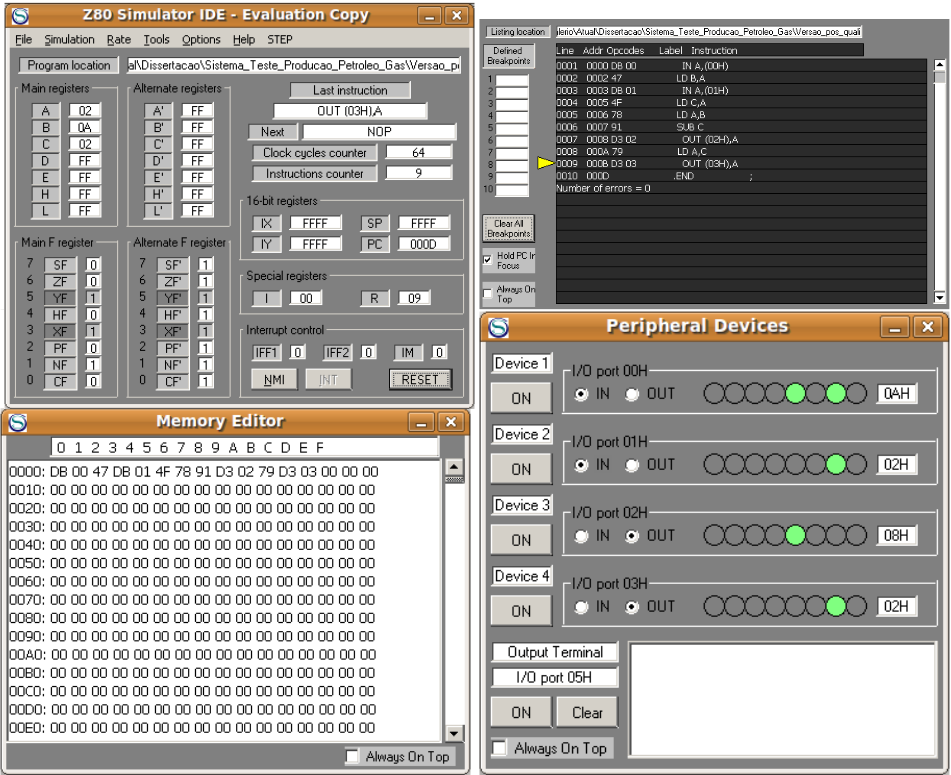
\includegraphics[width=1.0\textwidth]{images/Simulator_Full.png}
%\includegraphics[width=0.45\textwidth]{images/Simulator_Peripheral_Devices.png}
\caption{Window of Z80 simulator \cite{Simulator_z80}.}
\label{fig:simulacao}
\end{figure}

